%Author: Siddhesh Wani
%Date: January 4, 2016




\documentclass[12pt]{article}
\usepackage{tikz}
\usetikzlibrary{shapes.geometric, arrows}
\usepackage{hyperref}
\usepackage[a4paper]{geometry}
%DO NOT EDIT start
%Define different shapes to be used in flowchart
\tikzstyle{startstop} = [rectangle, rounded corners, minimum width=3cm, minimum height=1cm,text centered, draw=black, fill=red!30]
\tikzstyle{io} = [trapezium, trapezium left angle=70, trapezium right angle=110, minimum width=3cm, minimum height=1cm, text centered, draw=black, fill=blue!30]
\tikzstyle{process} = [rectangle, minimum width=3cm, minimum height=1cm, text centered, draw=black, fill=orange!30]
\tikzstyle{decision} = [diamond, minimum width=3cm, minimum height=1cm, text centered, draw=black, fill=green!30]
\tikzstyle{arrow} = [thick,->,>=stealth]
\tikzstyle{connector} = [signal,draw=black,fill=olive!30]%,text width=1cm,text height=1.5cm,align=center]
%DO NOT EDIT end




\begin{document}
\newgeometry{top=1cm, bottom=0.5cm,right=1cm,left=1.5cm}

\vspace*{2cm}
\begin{center} 


\section*{\hypertarget{updateSCI2CInfo}UpdateSCI2CInfo.sci}
{Siddhesh Wani}\\
 
\end{center}

\textbf{Introduction}\\
This fucntion gets next scilab function to be converted and updates its information in `Fileinfo' structure. 

\begin{center}
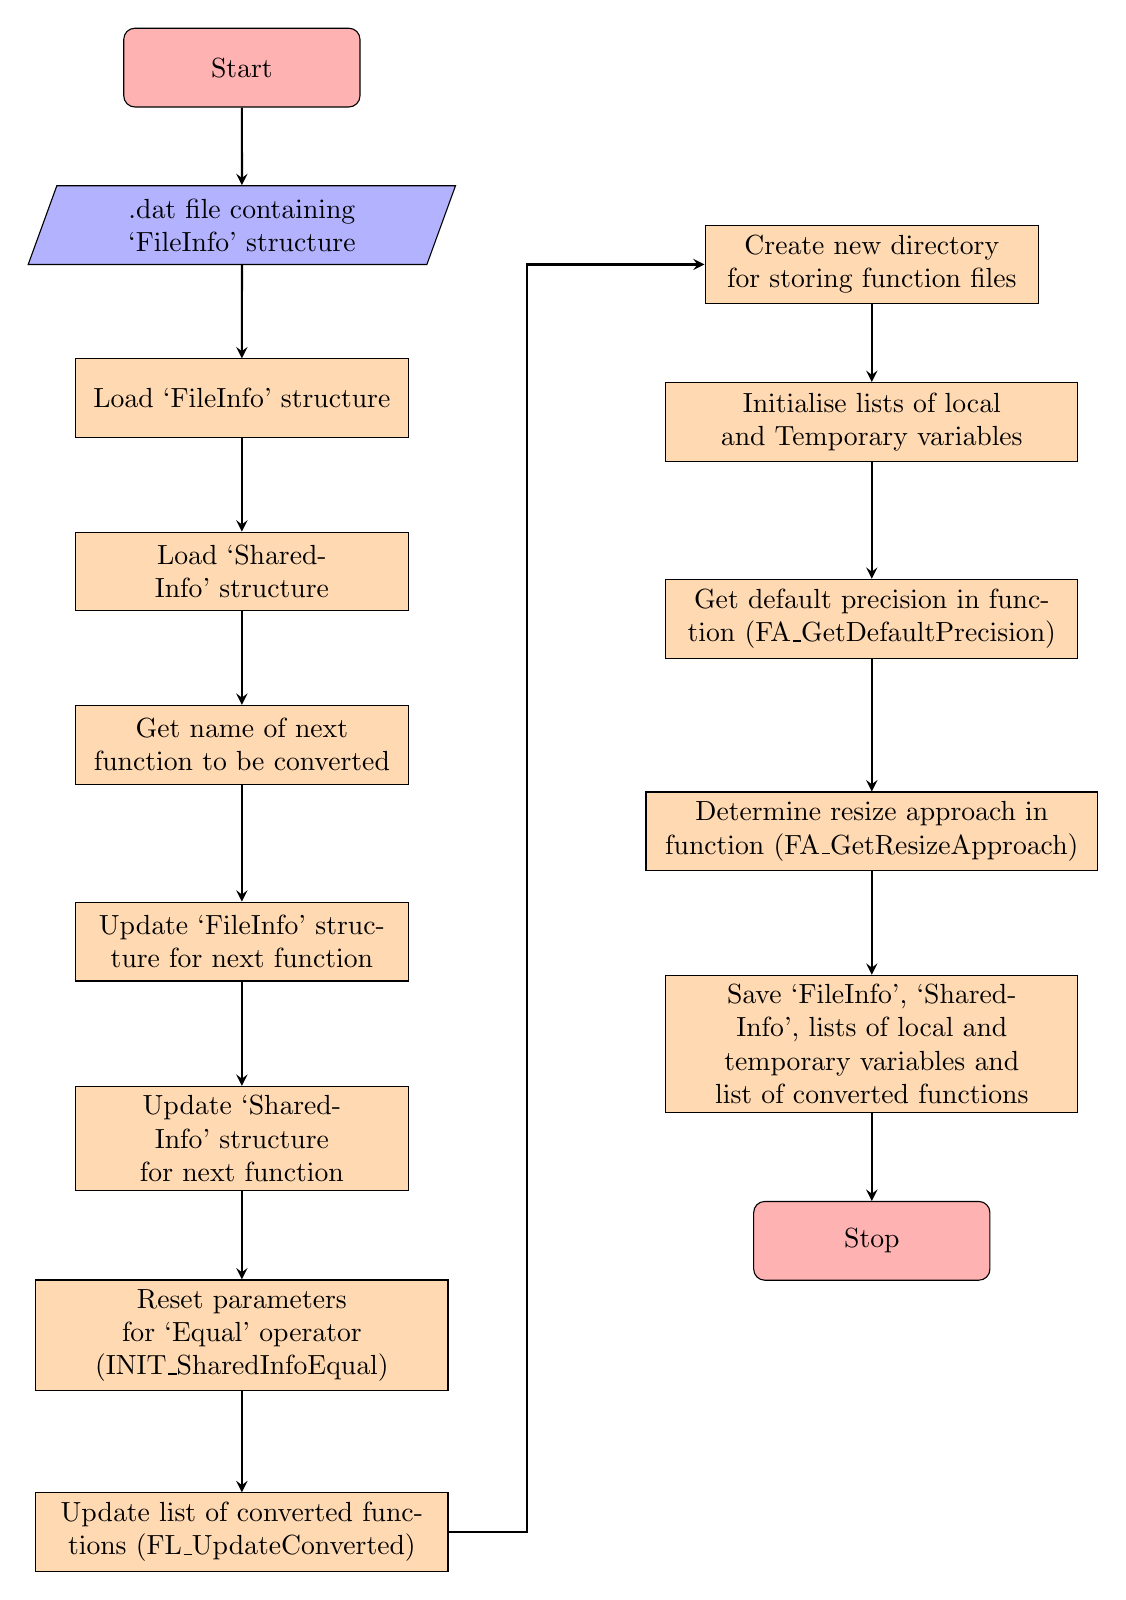
\begin{tikzpicture}[node distance=2cm]
\node (start) [startstop, xshift=-4cm] {Start};
\node (input) [io, below of=start, text width=4cm]{.dat file containing `FileInfo' structure};
\node (fileinfo)[process, below of=input, text width=4cm, yshift=-0.2cm]{Load `FileInfo' structure};
\node (sharedinfo)[process,below of=fileinfo, text width=4cm, yshift=-0.2cm]{Load `SharedInfo' structure};
\node (nextfun) [process, below of=sharedinfo, text width=4cm, yshift=-0.2cm]{Get name of next function to be converted};
\node (updfileinfo)[process, below of=nextfun, text width=4cm, yshift=-0.5cm]{Update `FileInfo' structure for next function};
\node (updsharedinfo)[process, below of=updfileinfo, text width=4cm, yshift=-0.5cm]{Update `SharedInfo' structure for next function};
\node (equal)[process, below of=updsharedinfo, text width=5cm, yshift=-0.5cm]{Reset parameters for `Equal' operator (INIT\_SharedInfoEqual)};
\node (converted)[process, below of=equal, text width=5cm, yshift=-0.5cm]{Update list of converted functions (FL\_UpdateConverted)};
\node (dir)[process, right of=input, text width=4cm, xshift=6cm, yshift=-0.5cm]{Create new directory for storing function files};
\node (temp) [process, below of=dir, text width=5cm]{Initialise lists of local and Temporary variables};
\node (precision)[process, below of=temp, text width=5cm, yshift=-0.5cm]{Get default precision in function (FA\_GetDefaultPrecision)};
\node (resize)[process, below of=precision, text width=5.5cm, yshift=-0.7cm]{Determine resize approach in function (FA\_GetResizeApproach)};
\node (save)[process, below of=resize, text width=5cm, yshift=-0.7cm]{Save `FileInfo', `SharedInfo', lists of local and temporary variables and list of converted functions};
\node (stop)[startstop, below of=save, yshift=-0.5cm]{Stop};

\draw [arrow] (start) -- (input);
\draw [arrow] (input) -- (fileinfo);
\draw [arrow] (fileinfo) -- (sharedinfo);
\draw [arrow] (sharedinfo) -- (nextfun);
\draw [arrow] (nextfun) -- (updfileinfo);
\draw [arrow] (updfileinfo) -- (updsharedinfo);
\draw [arrow] (updsharedinfo) -- (equal);
\draw [arrow] (equal) -- (converted);
\draw [arrow] (converted.east) --++(1cm,0) |- (dir.west);
\draw [arrow] (dir) -- (temp);
\draw [arrow] (temp) -- (precision);
\draw [arrow] (precision) -- (resize);
\draw [arrow] (resize) -- (save);
\draw [arrow] (save) -- (stop);





\end{tikzpicture}
\end{center}


\end{document}